\documentclass[a4paper,12pt]{article}

\usepackage[utf8]{inputenc}
\usepackage[T1]{fontenc}
\usepackage[a4paper,total={150mm,240mm}]{geometry}
\usepackage{amsmath}
\usepackage{amsfonts}
\usepackage{amsthm}
\usepackage{amscd}
\usepackage{grffile}
\usepackage{tikz}
\usepackage{eurosym}
\usepackage{graphicx}
\usepackage{color}
\usepackage{listings}
\lstset{language=C++, basicstyle=\ttfamily,
  keywordstyle=\color{black}\bfseries, tabsize=4, stringstyle=\ttfamily,
  commentstyle=\itshape, extendedchars=true, escapeinside={/*@}{@*/}}
\usepackage{paralist}
\usepackage{curves}
\usepackage{calc}
\usepackage{picinpar}
\usepackage{enumerate}
\usepackage{algpseudocode}
\usepackage{bm}
\usepackage{multibib}
\usepackage{hyperref}
\usepackage{textcase}
\usepackage{nicefrac}

\definecolor{listingbg}{gray}{0.95}

\title{DUNE PDELab Tutorial 03 \\
Conforming Finite Elements for a\\ Nonlinear Heat Equation}
\author{DUNE/PDELab Team}
\date{\today}

\begin{document}

\maketitle
\tableofcontents
\clearpage

\section{Introduction}

In this tutorial we extend the elliptic problem from tutorial 01 to the
time dependent case. Following the method of lines a general approach to time-dependent
problems is presented.

\subsection*{Depends On} This tutorial depends on tutorial 01.

\section{PDE Problem}

In this tutorial we consider the following problem:
\begin{align*}
\partial_t u -\Delta u + q(u) &= f &&\text{in $\Omega\times\Sigma$},\\
u &= g &&\text{on $\Gamma_D\subseteq\partial\Omega$},\\
-\nabla u\cdot \nu &= j &&\text{on $\Gamma_N=\partial\Omega\setminus\Gamma_D$},\\
u &= u_0 &&\text{at $t=0$}.
\end{align*}
This problem is a straightforward extension of the stationary
problem solved in tutorial 01.
The parameter functions $f$, $g$, $j$ may now also depend on time
and (with some restrictions) the subdivision into Dirichlet and Neumann boundary
can be time-dependent as well. The initial
condition $u_0$ is a function of $x\in\Omega$.

Multiplying with a test function and integrating in space
results in the following weak formulation \cite{Ern}:
Find $u\in L_2(t_0,t_0+T;u_g+V(t))$:
\begin{equation}
\frac{d}{dt} \int_\Omega u v \,dx+ \int_\Omega \nabla u \cdot \nabla v
+ q(u) v - f v \, dx + \int_{\Gamma_N} jv \, ds = 0 \qquad
\begin{array}{l}
\forall v \in V(t),\\
t \in \Sigma,
\end{array}
\label{eq:WeakForm}
\end{equation}
where $V(t) = \{v\in H^1(\Omega)\,:\, \text{$v=0$ on $\Gamma_D(t)$}\}$
and $H^1(\Omega)\ni u_g(t)|_{\Gamma_D}=g$. This can be written in a more compact way
with residual forms as follows:
\begin{equation*}
\frac{d}{dt} m^{\text{L2}}(u,v) + r^{\text{NLP}}(u,v) = 0 \quad \forall v \in V(t), t \in \Sigma.
\end{equation*}
where
\begin{equation*}
m^{\text{L2}}(u,v) = \int_\Omega u v \,dx
\end{equation*}
is the new temporal residual form, actually the $L_2$ inner product, and
\begin{equation*}
r^{\text{NLP}}(u,v) = \int_\Omega \nabla u \cdot \nabla v + (q(u)-f)v\,dx + \int_{\Gamma_N} jv\,ds ,
\end{equation*}
is the spatial residual form known from tutorial 01.
Under suitable assumptions it can be shown that problem \eqref{eq:WeakForm} has
a unique solution, see \cite{Ern} for the linear case.

\section{Finite Element Method}

In order to arrive at a fully discrete formulation we follow the method of lines
paradigm:
\begin{enumerate}[1)]
\item Choose a finite-dimensional test space $V_h(t)\subset V(t)$. Then \eqref{eq:WeakForm}
results in a system of ordinary differential equations for the coefficients $z_j(t)$
in the expansion of $u_h(t)=\sum_{j=1}^n (z_j(t))_j \phi_j$.
\item Choose an appropriate method to integrate the system of ordinary differential equations (ODEs).
\end{enumerate}

The finite-dimensional space we choose here is just the conforming
finite element space $V_h^{k,d}(\mathcal{T}_h,t)$ introduced in tutorial 01.
It may now depend also on time due to the time-dependent splitting of the boundary
in Dirichlet and Neumann part. Also the function $u_{h,g}(t)$ depends on time
and we have $u_h(t)\in U_h(t) = u_{h,g}(t) + V_h(t)$.

For the integration of the system of ODEs, subdivide the time interval into
not necessarily equidistant subintervals:
\begin{equation*}
\overline{\Sigma} = \{t^{0}\} \cup (t^0,t^1] \cup \ldots \cup (t^{N-1},t^N]
\end{equation*}
with $t^0=t_0$, $t^N=t_0+T$, $t^{k-1}<t^k$ for $1\leq k\leq N$ and
set  the time step to $\Delta t^k=t^{k+1}-t^k$.

One of the simplest ODE integrators is
the one-step-$\theta$ rule which reads:
\begin{equation}
\label{Eq:InstationaryProblem}
\begin{split}
&\text{Find $u_h^{k+1}\in U_h(t^{k+1})$ s.t.:}
\ \frac{1}{\Delta t_k}(m_h^\text{L2}(u_h^{k+1},v;t^{k+1})-m_h^\text{L2}(u_h^{k},v;t^{k})) + \\
&\hspace{25mm}\theta r_h^\text{NLP}(u_h^{k+1},v;t^{k+1}) + (1-\theta) r_h^\text{NLP}(u_h^{k},v;t^{k}) = 0
\quad \forall v\in V_h(t^{k+1}).
\end{split}
\end{equation}

Reordering terms shows that this method results in the solution
of a nonlinear system per time step which has the same structure as before:
\begin{equation*}
\text{Find $u_h^{k+1}\in U_h(t^{k+1})$ s.t.:}
\quad r_h^{\theta,k} (u_h^{k+1},v) + s_h^{\theta,k}(v) = 0
\quad \forall v\in V_h(t^{k+1}).
\end{equation*}
where
\begin{align*}
r^{\theta,k}_h(u,v) &= m_h^\text{L2}(u,v;t^{k+1})+\Delta t^k \theta r_h^\text{NLP}(u,v;t^{k+1}) ,\\
s^{\theta,k}_h(v) &= -m_h^\text{L2}(u^k_h,v;t^k) + \Delta t^k (1-\theta) r_h^\text{NLP}(u_h^k,v;t^k) .
\end{align*}
Implementation-wise the new residual form is comprised of a linear combination
of temporal and spatial residual forms.

The one step $\theta$ method results in the implicit Euler method for $\theta=1$,
the Crank-Nicolson method for $\theta=\nicefrac12$ and the explicit Euler method for $\theta=0$.
A large number of alternative methods are possible. In particular the class of
Runge-Kutta methods is introduced below.

\subsection*{Runge-Kutta Methods in Shu-Osher Form}

For the temporal and spatial residual forms $m_h$ and $r_h$, Runge-Kutta
methods can be written in the Shu-Osher form
\cite{shu_osher_88,gottlieb2011strong}:
\begin{enumerate}
\item $u_h^{(0)} = u_h^{k}$.
\item For $i=1,\ldots,s\in\mathbb{N}$, find $u_h^{(i)}\in u_{h,g}(t^k+d_i \Delta t^k)
+ V_h(t^{k+1})$:
\begin{equation*}
\begin{split}
\sum\limits_{j=0}^{s} \biggl[a_{ij} m_h&\left(u_h^{(j)},v;t^k+d_j \Delta t^k\right) \\
&\qquad + b_{ij} \Delta t^k r_h\left(u_h^{(j)}, v;t^k+d_j \Delta t^k\right) \biggr] = 0
\qquad \forall v\in V_h(t^{k+1}).
\end{split}
\end{equation*}
\item $u_h^{k+1} = u_h^{(s)}$.
\end{enumerate}
Here we assume that the same type of boundary condition
holds through the interval $(t^k,t^{k+1}]$. The parameter $s$ denotes
the number of stages of the scheme.
An $s$-stage scheme is given by the parameters
\begin{equation*}
A = \left[\begin{array}{ccc}
a_{10} & \ldots & a_{1s}\\
\vdots &  & \vdots\\
a_{s0} & \ldots & a_{ss}
\end{array}\right],
\quad B = \left[\begin{array}{ccc}
b_{10} & \ldots & b_{1s}\\
\vdots &  & \vdots\\
b_{s0} & \ldots & b_{ss}
\end{array}\right],
\quad d = \left(
d_{0}, \ldots, d_{s}
\right)^T.
\end{equation*}
\textit{Explicit} schemes are characterized by $a_{ij} = 0$ for $j>i$ and $b_{ij}=0$ for $j\geq i$.
\textit{Diagonally implicit} schemes are characterized by $a_{ij} = b_{ij}= 0$ for $j>i$.
Fully implicit schemes where $A$ and $B$ are full are not considered in PDELab.
Without loss of generality it can be assumed that $a_{ii}=1$. Moreover,
some diagonally implicit schemes, in particular all those implemented in PDELab right
now, satisfy $b_{ii}=b\,\forall i$. This means that in case of a linear problem the matrix is the
same in all steps and needs to be assembled only once.
PDELab allows you to add new schemes by specifying $A$, $B$ and $d$.
All explicit Runge-Kutta methods and most implicit Runge-Kutta methods
can be brought to the Shu-Osher form.
Some examples are:
\begin{itemize}
\item One step $\theta$ scheme (introduced above):
\begin{equation*}
A = \left[\begin{array}{cc}
-1 & 1
\end{array}\right],
\quad B = \left[\begin{array}{cc}
1-\theta & \theta
\end{array}\right],
\quad d = \left(
0, 1
\right)^T.
\end{equation*}
Explicit/implicit Euler ($\theta\in\{0,1\}$), Crank-Nicolson ($\theta=\nicefrac12$).
\item Heun's second order explicit method
\begin{equation*}
A = \left[\begin{array}{ccc}
-1 & 1 & 0\\
-\nicefrac12 & -\nicefrac12 & 1\\
\end{array}\right],
\quad B = \left[\begin{array}{ccc}
1 & 0 & 0\\
0 & \nicefrac12 & 0\\
\end{array}\right],
\quad d = \left(
0, 1, 1
\right)^T.
\end{equation*}
\item Alexander's two-stage second order strongly S-stable method \cite{alexander:77}:
\begin{equation*}
A = \left[\begin{array}{ccc}
-1 & 1 & 0\\
-1 & 0 & 1\\
\end{array}\right],
\quad B = \left[\begin{array}{ccc}
0 & \alpha     & 0\\
0 & 1-\alpha & \alpha\\
\end{array}\right],
\quad d = \left(
0, \alpha, 1
\right)^T
\end{equation*}
with $\alpha=1-\nicefrac{\sqrt{2}}{2}$.
\item Fractional step $\theta$ \cite{Meidner201545}, three stage second order strongly A-stable scheme:
\begin{equation*}
A = \left[\begin{array}{rrrr}
-1 & 1 & 0 & 0\\
0  & -1 & 1 & 0\\
0  & 0 & -1 & 1\\
\end{array}\right],
\quad B = \left[\begin{array}{rrrr}
\theta (1-\alpha) & \theta\alpha & 0 & 0\\
0 & \theta'\alpha & \theta' (1-\alpha) & 0\\
0 & 0 & \theta(1-\alpha) & \theta\alpha
\end{array}\right],
\quad d = \left(
0, \theta, 1-\theta, 1
\right)^T
\end{equation*}
with $\theta=1-\nicefrac{\sqrt{2}}{2}$, $\alpha=2\theta$, $\theta' = 1-2\theta = 1-\alpha = \sqrt{2}-1$.
Note also that $\theta\alpha= \theta' (1-\alpha) = 2\theta^2$.
\end{itemize}


\subsection*{Explicit Time Stepping Schemes}

Considering the case of the explicit Euler method ($\theta=0$) in \eqref{Eq:InstationaryProblem}
results in the problem: Find $u_h^{k+1}\in U_h(t^{k+1})$ s.t.:
\begin{equation*}
 m_h^\text{L2}(u_h^{k+1},v;t)-m_h^\text{L2}(u_h^{k},v;t) +
\Delta t^k r_h^\text{NLP}(u_h^{k},v;t) = 0
\quad \forall v\in V_h(t^{k+1}).
\end{equation*}
For certain spatial schemes, e.g. finite volume or discontinuous Galerkin,
and exploiting that $m_h^\text{L2}$ is bilinear, the corresponding algebraic system
to be solved is (block-) diagonal:
\begin{equation}
Dz^{k+1} = s^k - \Delta t^k q^k.
\end{equation}
Moreover, a stability condition restricting the time step $\Delta t^k$
has to be obeyed. The maximum allowable time step can be computed
explicitly for the simplest schemes and depends on the mesh $\mathcal{T}_h$.
For explicit time-stepping schemes therefore the following algorithm is employed:
\begin{enumerate}[i)]
\item While traversing the mesh assemble the vectors $s^k$ and
$q^k$ separately and compute the maximum time step $\Delta t^k$.
\item Form the right hand side $b^k=s^k - \Delta t^k q^k$ and ``solve'' the
diagonal system $Dz^{k+1} = b^k$ (can be done in one step).
\end{enumerate}
This procedure can be applied also to more general time-stepping schemes
such as strong stability preserving Runge-Kutta methods \cite{shu:88}.

\section{Realization in PDELab}

The structure of the code is very similar to that of tutorial 01.
It consists of the following files:
\begin{enumerate}[1)]
\item The ini-file
\lstinline{tutorial03.ini} holds parameters read by various parts of the code
which control the execution.
\item The main file \lstinline{tutorial03.cc} includes the necessary C++,
DUNE and PDELab header files
and contains the \lstinline{main} function where the execution starts.
The purpose of the \lstinline{main} function is
to instantiate DUNE grid objects and call the \lstinline{driver} function.
\item File \lstinline{driver.hh} instantiates the necessary PDELab classes
for solving a nonlinear instationary problem and finally solves the problem.
\item File \lstinline{nonlinearheatfem.hh} contains the local operator classes
\lstinline{NonlinearHeatFEM} and \lstinline{L2} realizing the spatial
and temporal residual forms.
\item File \lstinline{problem.hh} contains a parameter class which
encapsulates the user-definable part of the PDE problem.
\end{enumerate}

\subsection{Ini-File}

The ini-file contains a few new parameters compared to tutorial 01.
The \lstinline{fem} section contains a new parameter for the order of the
time stepping scheme (so 1 would be implicit Euler, 2 a second order
scheme like Alexander's 2 stage scheme):
\lstinputlisting[linerange={18-21},
basicstyle=\ttfamily\small,
frame=single,
backgroundcolor=\color{listingbg}]{../src/tutorial03.ini}
and the \lstinline{problem} section contains a parameter for the final time (the
initial time $t_0$ is always zero):
\lstinputlisting[linerange={23-25},
basicstyle=\ttfamily\small,
frame=single,
backgroundcolor=\color{listingbg}]{../src/tutorial03.ini}

\subsection{Function \lstinline{main}}

The \lstinline{main} function is very similar to the one in tutorial 01.
In order to simplify things only the structured grids \lstinline{OneDGrid}
and \lstinline{YaspGrid} are used.

\subsection{Parameter Class in \lstinline{problem.hh}}

The parameter class provides all data of the PDE problem: Coefficient functions,
boundary and initial conditions. They all may depend on time now in comparison to tutorial 01.
In order to pass the time argument there are at least two options:
\begin{enumerate}[1)]
\item Extend the interface of all methods by an additional time
argument.
\item Pass the evaluation time via a separate function and store the
time in a private data member for subsequent spatial evaluations.
\end{enumerate}
The second approach is taken in PDELab as it allows the reuse
of classes from the stationary case. Interfaces of methods are not changed
and only an additional method needs to be provided.
This new method on the class \lstinline{Problem} has the following implementation:
\lstinputlisting[linerange={63-67},
basicstyle=\ttfamily\small,
frame=single,
backgroundcolor=\color{listingbg}]{../src/problem.hh}
The method just stores the given time in
an internal data member.

The use of the time is shown by the Dirichlet boundary condition
extension method implementing the function
$u_g(x,t) = \sin(2\pi t)*\prod_{i=1}^{d-1} \sin^2(\pi x_i)\sin^2(10\pi x_i)$:
\lstinputlisting[linerange={43-54},
basicstyle=\ttfamily\small,
frame=single,
backgroundcolor=\color{listingbg}]{../src/problem.hh}
Note that there is no extra method for the initial condition.
The method \lstinline{g} is assumed to provide the initial condition
for the initial time.

\subsection{Function \lstinline{driver}}

We now go through the changes in the function \lstinline{driver} which
are due to instationarity. The first change concerns
the initialization of simulation time and set-up of the parameter object:
\lstinputlisting[linerange={14-17},
basicstyle=\ttfamily\small,
frame=single,
backgroundcolor=\color{listingbg}]{../src/driver.hh}

Now a PDELab grid function can be constructed:
\lstinputlisting[linerange={18-21},
basicstyle=\ttfamily\small,
frame=single,
backgroundcolor=\color{listingbg}]{../src/driver.hh}
A new function \lstinline{makeInstationaryGridFunctionFromCallable}
is provided since the grid function produced by it now also
provides a method \lstinline{setTime} to pass the time argument.
Note that the lambda closure and the parameter object need to be
provided as the \lstinline{setTime} method is only on the parameter class
and not on the lambda closure.

Setting up the grid function space and interpolating the initial condition
is the same as before. Then the grid operator for the spatial part can be
set up as in the stationary problem tutorial 01. We just use the new
local operator \lstinline{NonlinearHeatFEM}:
\lstinputlisting[linerange={54-61},
basicstyle=\ttfamily\small,
frame=single,
backgroundcolor=\color{listingbg}]{../src/driver.hh}

The temporal part is done similarly and just employs another local operator
\lstinline{L2}:
\lstinputlisting[linerange={62-66},
basicstyle=\ttfamily\small,
frame=single,
backgroundcolor=\color{listingbg}]{../src/driver.hh}

Spatial and temporal part are now combined using the
new class \lstinline{OneStepGridOperator} which can assemble
the linear combinations needed in the Runge-Kutta methods:
\lstinputlisting[linerange={67-68},
basicstyle=\ttfamily\small,
frame=single,
backgroundcolor=\color{listingbg}]{../src/driver.hh}

Linear solver backend and Newton method can be set up
in the same way as before, just using the \lstinline{OneStepGridOperator}.
Then a time-stepping scheme in the form of
the matrices $A$, $B$ and the vector $d$ introduced above needs to be selected.
Several classes are already provided and it is very easy to write your own class:
\lstinputlisting[linerange={80-82},
basicstyle=\ttfamily\small,
frame=single,
backgroundcolor=\color{listingbg}]{../src/driver.hh}

The selection mechanism for the time-stepping scheme
is implemented by setting a pointer to an appropriate method:
\lstinputlisting[linerange={83-90},
basicstyle=\ttfamily\small,
frame=single,
backgroundcolor=\color{listingbg}]{../src/driver.hh}
Note that \lstinline{TimeSteppingParameterInterface} is the interface from
which all time stepping parameter classes derive.

Then an object of class \lstinline{OneStepMethod} can be instantiated.
This class is able to compute a single time step of a general
Runge-Kutta one step method.
\lstinputlisting[linerange={91-93},
basicstyle=\ttfamily\small,
frame=single,
backgroundcolor=\color{listingbg}]{../src/driver.hh}

Before entering the time loop we set up VTK output for the instationary case.
Paraview has several ways to handle sequences of output files. Here we use
an advanced method that writes a special \lstinline{pvd}-file providing the
names of the files for each individual step and the associated absolute time. This
is particularly useful when non-equidistant time steps are used. All the
data files for the time steps are put in a subdirectory in order not to clog your file system.
The following code creates a directory (the name is read from the ini-file):
\lstinputlisting[linerange={101-110},
basicstyle=\ttfamily\small,
frame=single,
backgroundcolor=\color{listingbg}]{../src/driver.hh}

Now a \lstinline{SubsamplingVTKWriter} and a \lstinline{VTKSequenceWriter}
can be instantiated:
\lstinputlisting[linerange={106-111},
basicstyle=\ttfamily\small,
frame=single,
backgroundcolor=\color{listingbg}]{../src/driver.hh}
filled with data
\lstinputlisting[linerange={112-114},
basicstyle=\ttfamily\small,
frame=single,
backgroundcolor=\color{listingbg}]{../src/driver.hh}
and the first file is written
\lstinputlisting[linerange={115-115},
basicstyle=\ttfamily\small,
frame=single,
backgroundcolor=\color{listingbg}]{../src/driver.hh}

Now the time loop is under user control:
\lstinputlisting[linerange={118-136},
basicstyle=\ttfamily\small,
frame=single,
backgroundcolor=\color{listingbg}]{../src/driver.hh}
First the final time and time step are read from the parameter
file. Then, for each time step the constraints are reassembled. Note that
the boundary condition type is not supposed to
change \textit{within} a time step, so all stages of the Runge-Kutta Method
will use the same constraints (but not necessarily the same values at the
Dirichlet boundary).

Then, the \lstinline{apply} method of the one step method is used to
advance one step in time. Its arguments are the current \lstinline{time}, the
size of the time step \lstinline{dt}, the coefficient vector \lstinline{z} of the old
time step, the boundary condition function \lstinline{g} used to interpolate
boundary conditions for the stages and, as last argument, the new coefficient
vector \lstinline{znew} to be computed as a result.

In order to advance to the next time step the coefficient vector is copied and the
time variable is advanced. Finally, the output file for the time step is written.

Intentionally, the time loop is under user control to allow other things to be done,
e.g. choose adaptive time step size, proceeding to important absolute times,
writing only  every $n$th output file and so on.

\subsection{Spatial Local Operator}

The file \lstinline{nonlinearheatfem.hh} contains the two local operators
for the spatial and the temporal part. The class \lstinline{NonlinearHeatFEM} implements the
spatial part. It is actually very easy since the main part can be reused
from the \lstinline{NonlinearPoissonFEM} local operator  implemented in tutorial 01 through
public inheritance:
\lstinputlisting[linerange={25-42},
basicstyle=\ttfamily\small,
frame=single,
backgroundcolor=\color{listingbg}]{../src/nonlinearheatfem.hh}
Just a few methods need to be added to the local operator.
Default implementations can be inherited from
\lstinline{InstationaryLocalOperatorDefaultMethods}. Here only the method
\lstinline{setTime} needs to be implemented to pass on the time
to the parameter class for subsequent evaluations.

The following methods need to be provided by a local
operator for instationary computations:
\begin{lstlisting}[basicstyle=\ttfamily,
frame=single,
backgroundcolor=\color{listingbg}]
void setTime (R t_)
\end{lstlisting}
to set the time for all subsequent method calls.

\begin{lstlisting}[basicstyle=\ttfamily,
frame=single,
backgroundcolor=\color{listingbg}]
R getTime () const
\end{lstlisting}
to get the time set previously.

\begin{lstlisting}[basicstyle=\ttfamily,
frame=single,
backgroundcolor=\color{listingbg}]
void preStep (RealType time, RealType dt, int stages)
\end{lstlisting}
This method is called at the beginning of a time step, before all stages.

\begin{lstlisting}[basicstyle=\ttfamily,
frame=single,
backgroundcolor=\color{listingbg}]
void postStep ()
\end{lstlisting}
This method is called at the end of a time step, after all stages.

\begin{lstlisting}[basicstyle=\ttfamily,
frame=single,
backgroundcolor=\color{listingbg}]
void preStage (RealType time, int r)
\end{lstlisting}
This method is called at the beginning of a Runge-Kutta stage, where
$r$ is the number of the stage (starting with $r=1$).

\begin{lstlisting}[basicstyle=\ttfamily,
frame=single,
backgroundcolor=\color{listingbg}]
int getStage () const
\end{lstlisting}
Return the number of the current stage.

\begin{lstlisting}[basicstyle=\ttfamily,
frame=single,
backgroundcolor=\color{listingbg}]
void postStage ()
\end{lstlisting}
Called after the intermediate result of a stage has been computed.

\begin{lstlisting}[basicstyle=\ttfamily,
frame=single,
backgroundcolor=\color{listingbg}]
RealType suggestTimestep (RealType dt) const
\end{lstlisting}
In an explicit scheme this method can be called at the end of stage 1
to suggest a stable time step for the explicit scheme.

\subsection{Temporal Local Operator}

The temporal local operator needs to implement the
residual form related to the $L_2$-inner product. It could also
be used to compute an $L_2$ projection of some function.

Like in the spatial local operator we provide a finite element
map as template parameter and derive from some helpful
classes to provide default implementations of some methods:
\lstinputlisting[linerange={51-56},
basicstyle=\ttfamily\small,
frame=single,
backgroundcolor=\color{listingbg}]{../src/nonlinearheatfem.hh}

The following flag indicates that we provide a \lstinline{pattern_volume} method
specifying the sparsity pattern. Actually, this method is provided from the base class
\lstinline{FullVolumePattern}:
\lstinputlisting[linerange={64-64},
basicstyle=\ttfamily\small,
frame=single,
backgroundcolor=\color{listingbg}]{../src/nonlinearheatfem.hh}

The next flag indicates that just volume integrals depending
on trial and test functions are required:
\lstinputlisting[linerange={67-67},
basicstyle=\ttfamily\small,
frame=single,
backgroundcolor=\color{listingbg}]{../src/nonlinearheatfem.hh}

The implementation of \lstinline{alpha_volume}
is very similar to the reaction term in tutorial 01. For efficiency reasons
also \lstinline{jacobian_volume} is provided as well as the
\lstinline{*_apply_*} variants for matrix-free operation (which might
be very useful here since the mass matrix is well conditioned).

\subsection{Running the Example}

\begin{figure}
\begin{center}
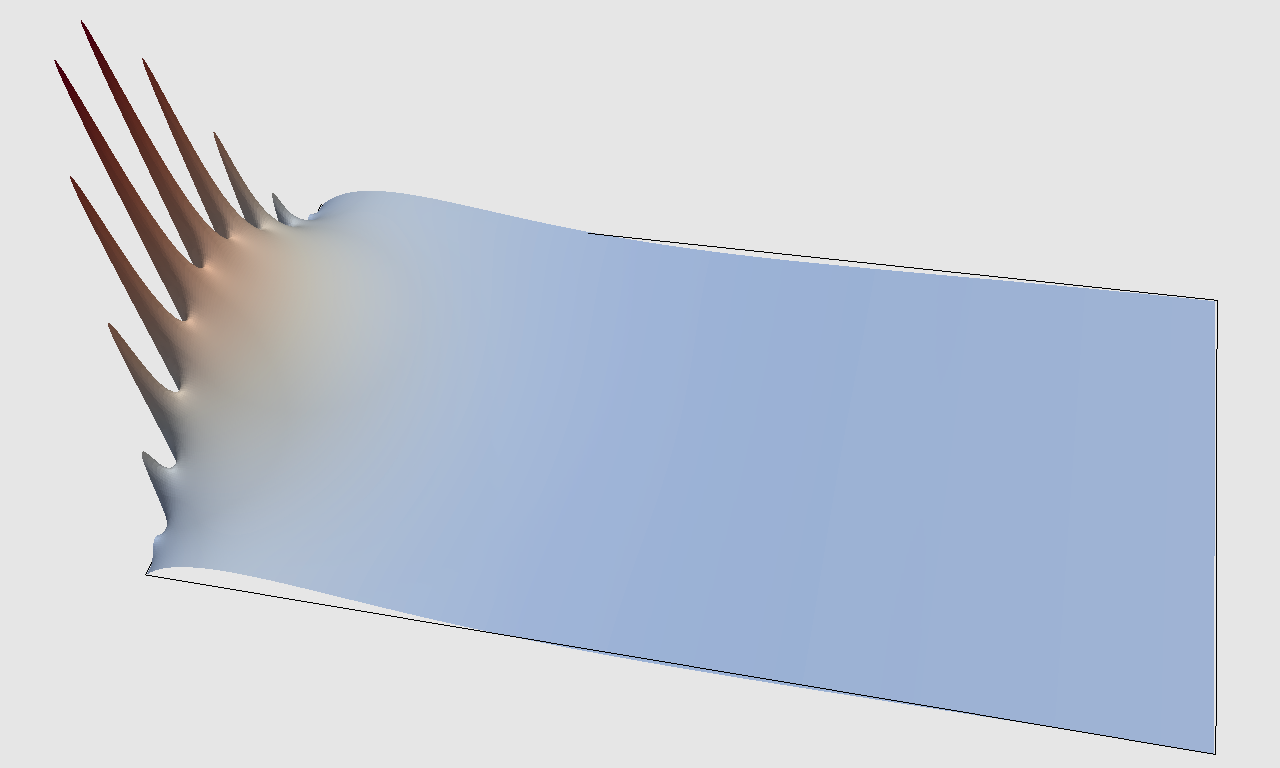
\includegraphics[width=0.9\textwidth]{warp}
\end{center}
\caption{Solution of the nonlinear heat equation.}
\label{fig:Bunt}
\end{figure}

The example solves the nonlinear heat equation in 1, 2 and 3 space dimensions.
A two-dimensional result is illustrated in Figure \ref{fig:Bunt}. On the left boundary
$x=0$ a function depending on time $t$ and $y$-coordinate is given, all the other
boundaries are of Neumann type with zero flux. The solution exhibits the
typical smoothing effect of parabolic problems in space and time.

\section{Outlook}

Several ideas could be pursued from this example:
\begin{itemize}
\item Experiment with a rough initial condition, observe
smoothing effect in time.
\item Explore the monotonicity properties of the scheme by
providing discontinuous initial conditions and testing different
polynomial degrees and temporal orders.
\end{itemize}

% bibtex bibliography
\bibliographystyle{plain}
\bibliography{tutorial03.bib}

\end{document}
